% Template adapted from https://github.com/jgm/pandoc-templates/blob/master/default.latex
% To be used with XeLaTex in memoiR
%%%%%%%%%%%%%%%%%%%%%%%%%%%%%%%%%%%%%%%%%%%%%%%%%%%%%%%%%%%%%%%%%%%%%%%%%%%%%%%%%%%%%%%%%

% Options for packages loaded elsewhere
\PassOptionsToPackage{unicode=true}{hyperref}
\PassOptionsToPackage{hyphens}{url}
\PassOptionsToPackage{dvipsnames,svgnames*,x11names*}{xcolor}
% Right to left support


\documentclass[
  12pt,
  american,
  a4paper,
  extrafontsizes,onecolumn,openright
  ]{memoir}

% Double (or whatever) spacing

% Math
\usepackage{amssymb, amsmath}
% mathspec: arbitrary math fonts
\usepackage{unicode-math}
\defaultfontfeatures{Scale=MatchLowercase}
\defaultfontfeatures[\rmfamily]{Ligatures=TeX,Scale=1}

% Fonts
\usepackage{lmodern}
\usepackage{fontspec}
% Main font
% Specific sanserif font
% Specific monotype font
% Specific math font
% Chinese, Japanese, Corean fonts

% Use upquote for straight quotes in verbatim environments
\usepackage{upquote}
% Use microtype
\usepackage[]{microtype}
\UseMicrotypeSet[protrusion]{basicmath} % disable protrusion for tt fonts

% Verbatim in note

% Color links
\usepackage{xcolor}

% Strikeout

% Necessary for code chunks
\usepackage{color}
\usepackage{fancyvrb}
\newcommand{\VerbBar}{|}
\newcommand{\VERB}{\Verb[commandchars=\\\{\}]}
\DefineVerbatimEnvironment{Highlighting}{Verbatim}{commandchars=\\\{\}}
% Add ',fontsize=\small' for more characters per line
\usepackage{framed}
\definecolor{shadecolor}{RGB}{248,248,248}
\newenvironment{Shaded}{\begin{snugshade}}{\end{snugshade}}
\newcommand{\AlertTok}[1]{\textcolor[rgb]{0.94,0.16,0.16}{#1}}
\newcommand{\AnnotationTok}[1]{\textcolor[rgb]{0.56,0.35,0.01}{\textbf{\textit{#1}}}}
\newcommand{\AttributeTok}[1]{\textcolor[rgb]{0.77,0.63,0.00}{#1}}
\newcommand{\BaseNTok}[1]{\textcolor[rgb]{0.00,0.00,0.81}{#1}}
\newcommand{\BuiltInTok}[1]{#1}
\newcommand{\CharTok}[1]{\textcolor[rgb]{0.31,0.60,0.02}{#1}}
\newcommand{\CommentTok}[1]{\textcolor[rgb]{0.56,0.35,0.01}{\textit{#1}}}
\newcommand{\CommentVarTok}[1]{\textcolor[rgb]{0.56,0.35,0.01}{\textbf{\textit{#1}}}}
\newcommand{\ConstantTok}[1]{\textcolor[rgb]{0.00,0.00,0.00}{#1}}
\newcommand{\ControlFlowTok}[1]{\textcolor[rgb]{0.13,0.29,0.53}{\textbf{#1}}}
\newcommand{\DataTypeTok}[1]{\textcolor[rgb]{0.13,0.29,0.53}{#1}}
\newcommand{\DecValTok}[1]{\textcolor[rgb]{0.00,0.00,0.81}{#1}}
\newcommand{\DocumentationTok}[1]{\textcolor[rgb]{0.56,0.35,0.01}{\textbf{\textit{#1}}}}
\newcommand{\ErrorTok}[1]{\textcolor[rgb]{0.64,0.00,0.00}{\textbf{#1}}}
\newcommand{\ExtensionTok}[1]{#1}
\newcommand{\FloatTok}[1]{\textcolor[rgb]{0.00,0.00,0.81}{#1}}
\newcommand{\FunctionTok}[1]{\textcolor[rgb]{0.00,0.00,0.00}{#1}}
\newcommand{\ImportTok}[1]{#1}
\newcommand{\InformationTok}[1]{\textcolor[rgb]{0.56,0.35,0.01}{\textbf{\textit{#1}}}}
\newcommand{\KeywordTok}[1]{\textcolor[rgb]{0.13,0.29,0.53}{\textbf{#1}}}
\newcommand{\NormalTok}[1]{#1}
\newcommand{\OperatorTok}[1]{\textcolor[rgb]{0.81,0.36,0.00}{\textbf{#1}}}
\newcommand{\OtherTok}[1]{\textcolor[rgb]{0.56,0.35,0.01}{#1}}
\newcommand{\PreprocessorTok}[1]{\textcolor[rgb]{0.56,0.35,0.01}{\textit{#1}}}
\newcommand{\RegionMarkerTok}[1]{#1}
\newcommand{\SpecialCharTok}[1]{\textcolor[rgb]{0.00,0.00,0.00}{#1}}
\newcommand{\SpecialStringTok}[1]{\textcolor[rgb]{0.31,0.60,0.02}{#1}}
\newcommand{\StringTok}[1]{\textcolor[rgb]{0.31,0.60,0.02}{#1}}
\newcommand{\VariableTok}[1]{\textcolor[rgb]{0.00,0.00,0.00}{#1}}
\newcommand{\VerbatimStringTok}[1]{\textcolor[rgb]{0.31,0.60,0.02}{#1}}
\newcommand{\WarningTok}[1]{\textcolor[rgb]{0.56,0.35,0.01}{\textbf{\textit{#1}}}}

% Listings package

% Tables
\usepackage{longtable,booktabs,tabu}
% Fix footnotes in tables (requires footnote package)
\IfFileExists{footnote.sty}{\usepackage{footnote}\makesavenoteenv{longtable}}{}

% Graphics
\usepackage{graphicx,grffile}
\graphicspath{{images/}}
\makeatletter
\def\maxwidth{\ifdim\Gin@nat@width>\linewidth\linewidth\else\Gin@nat@width\fi}
\def\maxheight{\ifdim\Gin@nat@height>\textheight\textheight\else\Gin@nat@height\fi}
\makeatother
% Scale images if necessary, so that they will not overflow the page
% margins by default, and it is still possible to overwrite the defaults
% using explicit options in \includegraphics[width, height, ...]{}
\setkeys{Gin}{width=\maxwidth,height=\maxheight,keepaspectratio}

% Prevent overfull lines
\setlength{\emergencystretch}{3em}  
\providecommand{\tightlist}{%
  \setlength{\itemsep}{0pt}\setlength{\parskip}{0pt}}

% Number sections for memoir (secnumdepth counter is ignored)
\setsecnumdepth{section}

% Set default figure placement to htbp
\makeatletter
\def\fps@figure{htbp}
\makeatother

% Include headers (preamble.tex) here
% Add LaTeX code into the preamble of the document here
\hyphenation{bio-di-ver-si-ty sap-lings}


%%%%%%%%%%%%%%%%%%%%%%%%%%%%%%%%%%%%%%%%%%%%%%%%%%%%%%%%%%%%%%%%%%%%%%%%%
% memoiR dalef3 chapter style 
% https://ctan.crest.fr/tex-archive/info/latex-samples/MemoirChapStyles/MemoirChapStyles.pdf
\usepackage{soul}
\definecolor{nicered}{rgb}{.647,.129,.149}
\makeatletter
\newlength\dlf@normtxtw
\setlength\dlf@normtxtw{\textwidth}
\def\myhelvetfont{\def\sfdefault{mdput}}
\newsavebox{\feline@chapter}
\newcommand\feline@chapter@marker[1][4cm]{%
  \sbox\feline@chapter{%
    \resizebox{!}{#1}{\fboxsep=1pt%
	  \colorbox{nicered}{\color{white}\bfseries\sffamily\thechapter}%
	}}%
  \rotatebox{90}{%
    \resizebox{%
	  \heightof{\usebox{\feline@chapter}}+\depthof{\usebox{\feline@chapter}}}%
	{!}{\scshape\so\@chapapp}}\quad%
  \raisebox{\depthof{\usebox{\feline@chapter}}}{\usebox{\feline@chapter}}%
 }
\newcommand\feline@chm[1][4cm]{%
  \sbox\feline@chapter{\feline@chapter@marker[#1]}%
  \makebox[0pt][l]{% aka \rlap
    \makebox[1cm][r]{\usebox\feline@chapter}%
  }}
\makechapterstyle{daleif1}{
  \renewcommand\chapnamefont{\normalfont\Large\scshape\raggedleft\so}
  \renewcommand\chaptitlefont{\normalfont\huge\bfseries\scshape\color{nicered}}
  \renewcommand\chapternamenum{}
  \renewcommand\printchaptername{}
  \renewcommand\printchapternum{\null\hfill\feline@chm[2.5cm]\par}
  \renewcommand\afterchapternum{\par\vskip\midchapskip}
  \renewcommand\printchaptertitle[1]{\chaptitlefont\raggedleft ##1\par}
}
\makeatother
\usepackage{booktabs}
\usepackage{longtable}
\usepackage{array}
\usepackage{multirow}
\usepackage{wrapfig}
\usepackage{float}
\usepackage{colortbl}
\usepackage{pdflscape}
\usepackage{tabu}
\usepackage{threeparttable}
\usepackage{threeparttablex}
\usepackage[normalem]{ulem}
\usepackage{makecell}
\usepackage{xcolor}

% Spacing in lists
\usepackage{enumitem}

% Polyglossia
\usepackage{polyglossia}
\setmainlanguage{en-US}
\setotherlanguage{fr-FR}
\setotherlanguage{it}

% BibLaTeX
\usepackage[backend=biber,style=authoryear-ibid,isbn=false,backref=true,giveninits=true,uniquename=init,maxcitenames=2,maxbibnames=150,sorting=nyt,sortcites=false]{biblatex}
\addbibresource{biblio/references.bib}

% cslreferences environment required by pandoc > 2.7



%%%%%%%%%%%%%%%%%%%%%%%%%%%%%%%%%%%%%%%%%%%%%%%%%%%%%%%%%%
% memoiR format

% Chapter Summary environment 
\usepackage[tikz]{bclogo}
\newenvironment{Summary}
  {\begin{bclogo}[logo=\bctrombone, noborder=true, couleur=lightgray!50]{In a Nutshell}\parindent0pt}
  {\end{bclogo}}
% Syntax:
%
%```{block, type='Summary'}
% Deliver message here.
% ```

% scriptsize code 
\let\oldverbatim\verbatim
\def\verbatim{\oldverbatim\scriptsize}
% Applies to code blocks and R code results
% code chunk options size='scriptsize' applies only to R code and results
% if the code chunk sets a different size, \def\verbatim{...} is prioritary for code results 


% Layout
%%%%%%%%%%%%%%%%%%%%%%%%%%%%%%%%%%%%%%%%%%%%%%%%%%%%%%%%%%

% Based on memoir, style companion
\newcommand{\MemoirChapStyle}{daleif1}
\newcommand{\MemoirPageStyle}{Ruled}

% Space between paragraphs
\usepackage{parskip}
	\abnormalparskip{3pt}

% Adjust margin paragraphs vertical position
\usepackage{marginfix}


% Margins
%%%%%%%%%%%%%%%%%%%%%%%%%%%%%%%%%%%%%%%

% allow use of '-',+','/' ans '*' to make simple length computation
\usepackage{calc}

% Full-width figures utilities
\newlength\widthw % full width
\newlength{\rf}
\newcommand*{\definesHSpace}{
  \strictpagecheck % slower but efficient detection of odd/even pages
  \checkoddpage
  \ifoddpage
  \setlength{\rf}{0mm}
  \else
  \setlength{\rf}{\marginparsep+\marginparwidth}
  \fi
}

\makeatletter
% 1" margins for the front matter.
\newcommand*{\SmallMargins}{
  \setlrmarginsandblock{1.5in}{1.5in}{*}
  \setmarginnotes{0.1in}{0.1in}{0.1in}
 \setulmarginsandblock{1.5in}{1in}{*}
  \checkandfixthelayout
  \ch@ngetext
  \clearpage
  \setlength{\widthw}{\textwidth+\marginparsep+\marginparwidth}
  \footnotesatfoot
  \chapterstyle{\MemoirChapStyle}	% Chapter and page styles must be recalled
  \pagestyle{\MemoirPageStyle}
}

% 3" outer margin for the main matter
\newcommand{\LargeMargins}{\SmallMargins}
\makeatother

% Figure captions and footnotes in outer margins


% Main title page with filigrane
%%%%%%%%%%%%%%%%%%%%%%%%%%%%%%%%%%%%%%%%%%%%%%%%%%%%%%%%%%

\newcommand{\MainTitlePage}[2]{
	\SmallMargins % Margins
	\pagestyle{empty} % No header/footer
	~\\ % Print a character or the page will not exist
	\begin{textblock}{2}(30,10)
		\rule{1pt}{\paperheight-20mm}
	\end{textblock}
	\begin{textblock}{140}(50, 45)
		\flushright
		\begin{Spacing}{3}
			{\fontfamily{qtm}\selectfont\fontsize{45}{45}\selectfont \textsc{\thetitle}}
		\end{Spacing}
	\end{textblock}
	\begin{textblock}{140}(50, 125)
		\flushright
		{\fontfamily{qtm}\Large \theauthor}
	\end{textblock}
		\begin{textblock}{140}[0, 1](50, 262)
		\normalfont	Version: \thedate
	\end{textblock}
	\newpage
	~\\ % Print a character or the page will not exist
	\begin{textblock}{140}(40, 40)
		#1
	\end{textblock}
	\begin{textblock}{140}[0,1](40, 270)
		\centering
    
\includegraphics[width=5cm]{logo}\\ \bigskip
    #2
	\end{textblock}
	\newpage
}

% Clear page and open an even one (\clearpage opens an odd one)
\newcommand{\evenpage}{
  \clearpage
	\strictpagecheck % slower but efficient detection of odd/even pages
  \checkoddpage
  \ifoddpage
    \thispagestyle{empty}
    ~\\ % Print a character or the page will not exist
    \newpage
  \else
    % do nothing
  \fi
}

% Text blocks
\usepackage[absolute,overlay]{textpos}
	\setlength{\TPHorizModule}{1mm}
	\setlength{\TPVertModule}{1mm}


%% PDF title page to insert
%%%%%%%%%%%%%%%%%%%%%%%%%%%%%%%%%%%%%%%%%%%%%%%%%%%%%%%%%%

\usepackage{pdfpages}


%% Bibliography
%%%%%%%%%%%%%%%%%%%%%%%%%%%%%%%%%%%%%%%%%%%%%%%%%%%%%%%%%%

\usepackage[strict,autostyle]{csquotes}
% Repeated citation as author-year-title instead of author-title (modification of footcite:note in verbose-inote.cbx)

%% Table of Contents
%%%%%%%%%%%%%%%%%%%%%%%%%%%%%%%%%%%%%%%%%%%%%%%%%%%%%%%%%%

% fix the typesetting of the part number
\renewcommand\partnumberlinebox[2]{#2\ ---\ }


% Fonts
%%%%%%%%%%%%%%%%%%%%%%%%%%%%%%%%%%%%%%%%%%%%%%%%%%%%%%%%%%


% Hyperref comes last
%%%%%%%%%%%%%%%%%%%%%%%%%%%%%%%%%%%%%%%%%%%%%%%%%%%%%%%%%%

\usepackage{hyperref}
\hypersetup{
  pdftitle={Memoir Template},
  pdfauthor={CEFE R users},
  colorlinks=true,
  linkcolor=Maroon,
  citecolor=Blue,
  urlcolor=Blue,
  breaklinks=true}

% Don't use monospace font for urls
\urlstyle{same}


% Title, author, date from YAML to LaTeX
%%%%%%%%%%%%%%%%%%%%%%%%%%%%%%%%%%%%%%%%%%%%%%%%%%%%%%%%%%

\title{Memoir Template}

\author{CEFE R users}

\date{2022-03-25}


% End of preamble
%%%%%%%%%%%%%%%%%%%%%%%%%%%%%%%%%%%%%%%%%%%%%%%%%%%%%%%%%%


\begin{document}
\frontmatter

% Title page
%%%%%%%%%%%%%%%%%%%%%%%%%%%%%%%%%%%%%%%%%%%%%%%%%%%%%%%%%%


\includepdf[pages=1]{images/cover.pdf}
\cleardoublepage

\MainTitlePage{This document is reproducible thanks to:

\begin{itemize}
  \item \LaTeX and its class memoir (\url{http://www.ctan.org/pkg/memoir}).
  \item R (\url{http://www.r-project.org/}) and RStudio (\url{http://www.rstudio.com/})
  \item bookdown (\url{http://bookdown.org/}) and memoiR (\url{https://ericmarcon.github.io/memoiR/})
\end{itemize}}{Name of the owner of the logo

\url{https://www.cefe.cnrs.fr/fr/}

An explanatory sentence.
Leave an empty line for line breaks.}


% Before Body
%%%%%%%%%%%%%%%%%%%%%%%%%%%%%%%%%%%%%%%%%%%%%%%%%%%%%%%%%%





% Contents
%%%%%%%%%%%%%%%%%%%%%%%%%%%%%%%%%%%%%%%%%%%%%%%%%%%%%%%%%%

\LargeMargins
{
\hypersetup{linkcolor=}
\setcounter{tocdepth}{2}
\tableofcontents
}


% Body
%%%%%%%%%%%%%%%%%%%%%%%%%%%%%%%%%%%%%%%%%%%%%%%%%%%%%%%%%%

\LargeMargins
\mainmatter

\hypertarget{notes-atelier-rmarkdown}{%
\chapter{Notes Atelier Rmarkdown}\label{notes-atelier-rmarkdown}}

Autrices et auteurs :

\begin{itemize}
\tightlist
\item
  Joris Huguenin
\item
  Clara Gritti
\item
  Camila Leandro
\item
  Nathalie Zeballos
\item
  Océane Cobelli
  Ce document est une prise de notes collaboratives de l'atelier Rmarkdown effectué au CEFE le 25 mars 2022.
\end{itemize}

\hypertarget{pourquoi-utiliser-rmarkdown}{%
\section{Pourquoi utiliser Rmarkdown ?}\label{pourquoi-utiliser-rmarkdown}}

Utiliser word, notamment pour des documents longs et complexes, peut rapidement être plus couteux en termes d'effort.

\url{https://bookdown.org/yihui/rmarkdown/}

WISYMIG \& WISYMIM (sont sur un bâteau ? ) What you see is what you get (word, openoffice) VS What you see is what you mean (Rmarkdown). Sous R, nous pouvons écrire un script qui peut être exporté en .rmd. La fonction knitr (petit bouton sous Rstudio avec une pelotte de laine) permet ensuite de compiler et exporter sous différents formats (.tex (et .pdf), .docx, .html).

Pour plus d'informations \url{https://stateofther.github.io/finistR2018/atelier3_advancedrmd.html}

\url{https://ismayc.github.io/rbasics-book/5-rmdanal.html}

Avantage d'utiliser le package memoiR au lieu de simplement Markdown: Création d'un ensemble de fichiers (cf plus bas) pour gérer plus facilement des documents plus longs/complexes (thèse, livre), avec un fichier rmd par chapitre (gain de temps pour knitter, interchanger position des chp etc).

\hypertarget{profil-des-utilisateurs-de-latelier}{%
\section{Profil des utilisateurs de l'atelier}\label{profil-des-utilisateurs-de-latelier}}

\begin{itemize}
\tightlist
\item
  scripts R : 8 TB / 5 BOF {[}sur 13 partcipants{]}
\item
  projets R : 10 oui /3 non {[}Joris nous parle importance de faire des projets à chaque début de projet, notamment pour l'utilisation de Git{]}
\item
  Git (Github, GitLab, \ldots) : 4 {[}le CNRS va déployer un GitLab{]}
\item
  BibTex : 10 oui / 3 non {[}Logiciels type Zotero,\ldots{} // memoiR utilise très bien les documents .bib{]}
\item
  Rmarkdown : 8.5 oui / 4.5 non
\item
  LaTeX : 1 oui / 12 non
\item
  Beamer : {[}outil pour construire des présentations ; avantages : facile à faire / désaventages : moins intuitif que powerpoint{]}
\item
  MemoiR : personne ne l'a déjà utilisé
\end{itemize}

\hypertarget{compilation-dans-rstudio}{%
\section{Compilation dans Rstudio}\label{compilation-dans-rstudio}}

Écrire un fichier .rmd avec un peu de texte, de l'import de data, et un résultat sous forme de tableau ou graphe.

Déposer les fichiers .rmd ici : \url{https://mycore.core-cloud.net/index.php/s/cdMB0VkkrYplVk3} et les annexes dans les dossiers correspondants.

\hypertarget{le-fichier-.rmd}{%
\subsection{Le fichier .rmd}\label{le-fichier-.rmd}}

La cheatsheet : \url{https://www.rstudio.com/wp-content/uploads/2015/02/rmarkdown-cheatsheet.pdf}

Le guide de référence : \url{https://www.rstudio.com/wp-content/uploads/2015/03/rmarkdown-reference.pdf}

\hypertarget{comment-guxe9re-t-on-la-bibliographie}{%
\subsection{Comment gére-t-on la bibliographie ?}\label{comment-guxe9re-t-on-la-bibliographie}}

citr : package pour faire sa bibliographie (une recherche du nom de l'auteur permet d'insérer la réfernce). Pour en savoir plus : \url{https://github.com/crsh/citr} Après l'installation du package, il peut être nécessaire de quitter/rouvrir le projet pour que l'option ``Insert citation'' apparaisse dans le volet de ``Addins''. /!~Le package peut ne pas être disponible pour certaines versions de R.

On n'est pas obligé d'installer citr si on a précisé le fichier .bib dans le YAML, on peut utiliser @\ldots{} (fonctionne en mode ``compas'', pas en mode ``normal''). Avec le @, on accède au .bib et à la bibliothèque principale de zotero.

Aternative, utiliser les clés de citation bibTex avec les logiciels de gestion de bibliographie :

Zotero -\textgreater{} extension Better BibTex {[}\url{https://retorque.re/zotero-better-bibtex/}{]}, crée une clé de citation pour chaque biblio -\textgreater{} extraction d'un fichier bibtex lu par R (fichier .bib en UTF-8) -\textgreater{} on le range dans un dossier /biblio dans notre projet R -\textgreater{} pour l'importer dans le fichier Rmd on écrit dans l'en-tête du document (YAML) : ``bibliography : biblio/nomdufichier.bib'' ; on peut aussi ajouter des options pour les citations avec biblatexoptions

Pour Mendeley il y a cette aide en ligne \url{https://blog.mendeley.com/2011/10/25/howto-use-mendeley-to-create-citations-using-latex-and-bibtex/}. Sinon sélectionner les citations qui vous intéressent (CTRL + A sélectionne tout dans le dossier choisi), puis Edit -\textgreater{} Exporter.

Le choix du style de citations peut se faire dans les options au début.

\hypertarget{yaml}{%
\subsection{YAML ?}\label{yaml}}

Partie du haut qui donne les caractéristiques générales du document (titre, auteur, date, gestion de la bibliographie\ldots).

\hypertarget{chunck}{%
\subsection{chunck ?}\label{chunck}}

\url{https://yihui.org/knitr/options/\#cache}

Pour mettre du code dans le document

Il est possible d'utiliser le raccourci ctrl+alt+i pour insérer rapidement un chunk.

\hypertarget{la-gestion-du-cache}{%
\subsection{la gestion du cache}\label{la-gestion-du-cache}}

Dans un premier ``chunk'' qui peut s'appeler \emph{setup }on peut ajouter un certain nombre de directives pour l'ensemble des chunks. Par exemple, comment afficher à chaque fois les images. Pour le cache c'est ici qu'on va introduire deux paramètres, qui permettent que le calcul se fasse qu'une seule fois et que le résultat soit enregistré, ainsi lors d'une prochaine compilation, il n'y pas nécessité de tout recalculer (ça fait gagner du temps !).

\begin{itemize}
\item
  cache = TRUE
\item
  cache.lazy = FALSE)
\end{itemize}

\url{https://bioinfo-fr.net/maitrisez-cache-de-rmarkdown}

\hypertarget{mise-en-page}{%
\subsection{Mise en page}\label{mise-en-page}}

Visualier le rendu sans knitter : petite icone compas en haut à droite (``Switch to visual markdown editor'').

** blablabla ** --\textgreater{} rendu en gras : \textbf{blablabla}

`mean(data\$colonneA)' --\textgreater{} sort le résultat de la fonction demandée, ici la moyenne de la colonne A du fichier data

\hypertarget{et-les-tableaux}{%
\subsection{Et les tableaux ?}\label{et-les-tableaux}}

avec kable, kableExtra et flextable

kable = le package de base pour afficher des tableaux

kableExtra = package amélioré qui permet de mettre en forme les tableaux

\hypertarget{les-uxe9quations-mathuxe9matiques}{%
\subsection{Les équations mathématiques ?}\label{les-uxe9quations-mathuxe9matiques}}

dans MemoiR : packages amsmaths et amssyms (?), chargés dans le template.tex

\hypertarget{uxe9crire-un-article}{%
\section{Écrire un article}\label{uxe9crire-un-article}}

Rmd -\textgreater{} from template {[}choix parmi un éventail (i.e.~PNAS, Plos, Elsevier publications\ldots{]}

install.packages(``rticles'')

library(rticles)

\url{https://pagedown.rbind.io/}

\hypertarget{uxe9crire-un-muxe9moire}{%
\section{Écrire un mémoire}\label{uxe9crire-un-muxe9moire}}

Nouveau projet -\textgreater{} Markdown (choisi memoiR -\textgreater{} document type memoir)

Beaucoup de fichier et dossiers se créent ; ça peut impressioner, mais ça veut juste dire qu'il a ``déjà travaillé''. Rien que compiler l'exemple permet d'avoir un guide pour créer son propre mémoire (ça prends plusieurs minutes).

Intérêt de faire des chapitres : mieux gérer un doc long (manuscrit de thèse par exemple), inverser ordre des chapitres rapidement (juste changer nom du fichier et R recompile dans le nouvel ordre), temps de compilation qui diminue.

chapitrer son document

Le référencement croisé

\url{https://ericmarcon.github.io/memoiR/gallery/memoir/bookdown_gitbook/index.html}

\url{https://ericmarcon.github.io/travailleR/} {[}Excellente référence pour travailler sur R (pas que sur Markdown){]}

Plusieurs fichiers créés, dont :

\begin{itemize}
\item
  index --\textgreater{} YAML que dans ce fichier (préciser page de garde créée en tant que pdf au préalable)

  \begin{itemize}
  \item
    \begin{itemize}
    \tightlist
    \item
      précision de la langue (pour accès aux accents etc), de l'abstract, des mots-clés dans ce fichier ; Il est en effet important de noter -langage: english (ou bien le langage utilisé dans le document)
    \end{itemize}
  \item
    \begin{itemize}
    \tightlist
    \item
      1er chunk : NE PAS MODIFIER !
    \end{itemize}
  \item
    \begin{itemize}
    \tightlist
    \item
      2ème chunk qui permet de gérer le style des figures
    \end{itemize}
  \item
    \begin{itemize}
    \tightlist
    \item
      3ème chunk : knitr options --\textgreater{} mettre la librairie ici
    \end{itemize}
  \item
    \begin{itemize}
    \tightlist
    \item
      Glossaire : permet de faire le lien avec les titres de nos différents chapitres
    \end{itemize}
  \item
    -unnumbered (ne pas commencer la pagination à cette section)
  \end{itemize}
\item
  syntax
\item
  getting start
\item
  etc.
\end{itemize}

Organisation de notre mémoire : le + efficace c'est de faire 1 fichier par chapitre, la numérotation des chapitres va permettre de compiler le tout dans le bon ordre (mais après, ça reste une préférence personnelle, on peut mettre tous les chapitres dans le même fichier si on préfére, ça sera un peu + long à compiler)

Références internes au document à mettre entre \{\}

Dans le sous-dossier latex

\begin{itemize}
\tightlist
\item
  template.tex -\textgreater{} package intégrés pour écrire des formules mathématiques, options pour la bibliographie, options gitbook avec titre et url personnels (researchgate\ldots)
\end{itemize}

Indiquer la langue qu'on utilise (dans template.tex) : sert à charger les bons caractères (notamment pour les accents) et possibilité d'avoir un correcteur orthographique

Template.tex = tout est déjà réglé en language LaTex, bien pratique si on veut juste modifier qqs options

\begin{itemize}
\tightlist
\item
  Fichiers after\_body.tex = pour ajouter des annexes en fin de rapport
\end{itemize}

Package tinytex : gère le langage LaTex dans R

\hypertarget{les-pinuxe8des}{%
\chapter{Les pinèdes}\label{les-pinuxe8des}}

\hypertarget{de-nos-ruxe9gions}{%
\section{de nos régions}\label{de-nos-ruxe9gions}}

C'est trop joli. Il y a plein de pins.

\begin{figure}
\centering
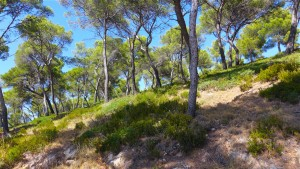
\includegraphics{images/pinede.jpg}
\caption{une image de pinède de pins d'Alep}
\end{figure}

Note de Joris : Attention, j'ai corrigé l'adresse de l'image. Puisque nous travaillons dans un projet, il faut juste écrire images/pinede.jpg et non pas C:/Users/c.gritti/Documents/CEFE\_book/\ldots{}

\hypertarget{e-partie-les-pollinisateurs-des-pins}{%
\chapter{2e partie : les pollinisateurs des pins}\label{e-partie-les-pollinisateurs-des-pins}}

\hypertarget{uxe7a-nexiste-pas}{%
\section{ça n'existe pas}\label{uxe7a-nexiste-pas}}

Par contre il y en a en dessous pour le romarin et le thym.

\scriptsize

\begin{Shaded}
\begin{Highlighting}[]
\FunctionTok{kable}\NormalTok{(export\_TAG\_3011\_net[}\DecValTok{1}\SpecialCharTok{:}\DecValTok{10}\NormalTok{, }\FunctionTok{c}\NormalTok{(}\DecValTok{24}\NormalTok{, }\DecValTok{73}\NormalTok{, }\DecValTok{83}\NormalTok{)], }\AttributeTok{align =} \StringTok{"c"}\NormalTok{) }\SpecialCharTok{\%\textgreater{}\%}
    \FunctionTok{kable\_styling}\NormalTok{(}\AttributeTok{latex\_options =} \StringTok{"striped"}\NormalTok{)}
\end{Highlighting}
\end{Shaded}

\begin{table}
\centering
\begin{tabular}{c|c|c}
\hline
commune & nom\_reconnu & abondance\\
\hline
\cellcolor{gray!6}{Gruissan} & \cellcolor{gray!6}{Smilax aspera L., 1753} & \cellcolor{gray!6}{\vphantom{1} P}\\
\hline
Gruissan & Quercus ilex L., 1753 & 1\\
\hline
\cellcolor{gray!6}{Gruissan} & \cellcolor{gray!6}{Smilax aspera L., 1753} & \cellcolor{gray!6}{P}\\
\hline
Gruissan & Aphyllanthes monspeliensis L., 1753 & 1\\
\hline
\cellcolor{gray!6}{Gruissan} & \cellcolor{gray!6}{Quercus ilex L., 1753} & \cellcolor{gray!6}{P}\\
\hline
Gruissan & Aphyllanthes monspeliensis L., 1753 & P\\
\hline
\cellcolor{gray!6}{Leucate} & \cellcolor{gray!6}{Quercus ilex L., 1753} & \cellcolor{gray!6}{P}\\
\hline
Leucate & Sedum sediforme (Jacq.) Pau, 1909 & P\\
\hline
\cellcolor{gray!6}{Leucate} & \cellcolor{gray!6}{Smilax aspera L., 1753} & \cellcolor{gray!6}{P}\\
\hline
Leucate & Helichrysum stoechas (L.) Moench, 1794 & P\\
\hline
\end{tabular}
\end{table}

\normalsize

\scriptsize

\begin{Shaded}
\begin{Highlighting}[]
\FunctionTok{library}\NormalTok{(sp)}
\FunctionTok{library}\NormalTok{(raster)}
\FunctionTok{library}\NormalTok{(rgdal)}
\CommentTok{\# install.packages(\textquotesingle{}Rtools\textquotesingle{}) install.packages(\textquotesingle{}citr\textquotesingle{})}
\CommentTok{\# install.packages(\textquotesingle{}devtools\textquotesingle{}) library(devtools)}
\CommentTok{\# devtools::install\_github(\textquotesingle{}crsh/citr\textquotesingle{}) library(citr)}
\end{Highlighting}
\end{Shaded}

\normalsize

\hypertarget{aperuxe7u-des-donnuxe9es}{%
\chapter{Aperçu des données}\label{aperuxe7u-des-donnuxe9es}}

Nous avons un raster d'altitude à 25m pour la région des Alpes du Sud, téléchargé depuis le site de l'IGN \autocite{ign_rge_2013}.

\scriptsize

\begin{Shaded}
\begin{Highlighting}[]
\CommentTok{\# data = read\_excel(\textquotesingle{}data/releves\_genepi\_2021.xlsx\textquotesingle{}, sheet}
\CommentTok{\# = 2)}
\NormalTok{raster }\OtherTok{=} \FunctionTok{raster}\NormalTok{(}\StringTok{"data/MNT25\_PNM.tif"}\NormalTok{)}
\CommentTok{\# limites = readOGR(\textquotesingle{}data/pn2008.shp\textquotesingle{}) crs(limites) =}
\CommentTok{\# CRS(\textquotesingle{}EPSG:2154\textquotesingle{})}
\end{Highlighting}
\end{Shaded}

\normalsize

Ce raster peut être visualisé ci-dessous.

\scriptsize

\begin{center}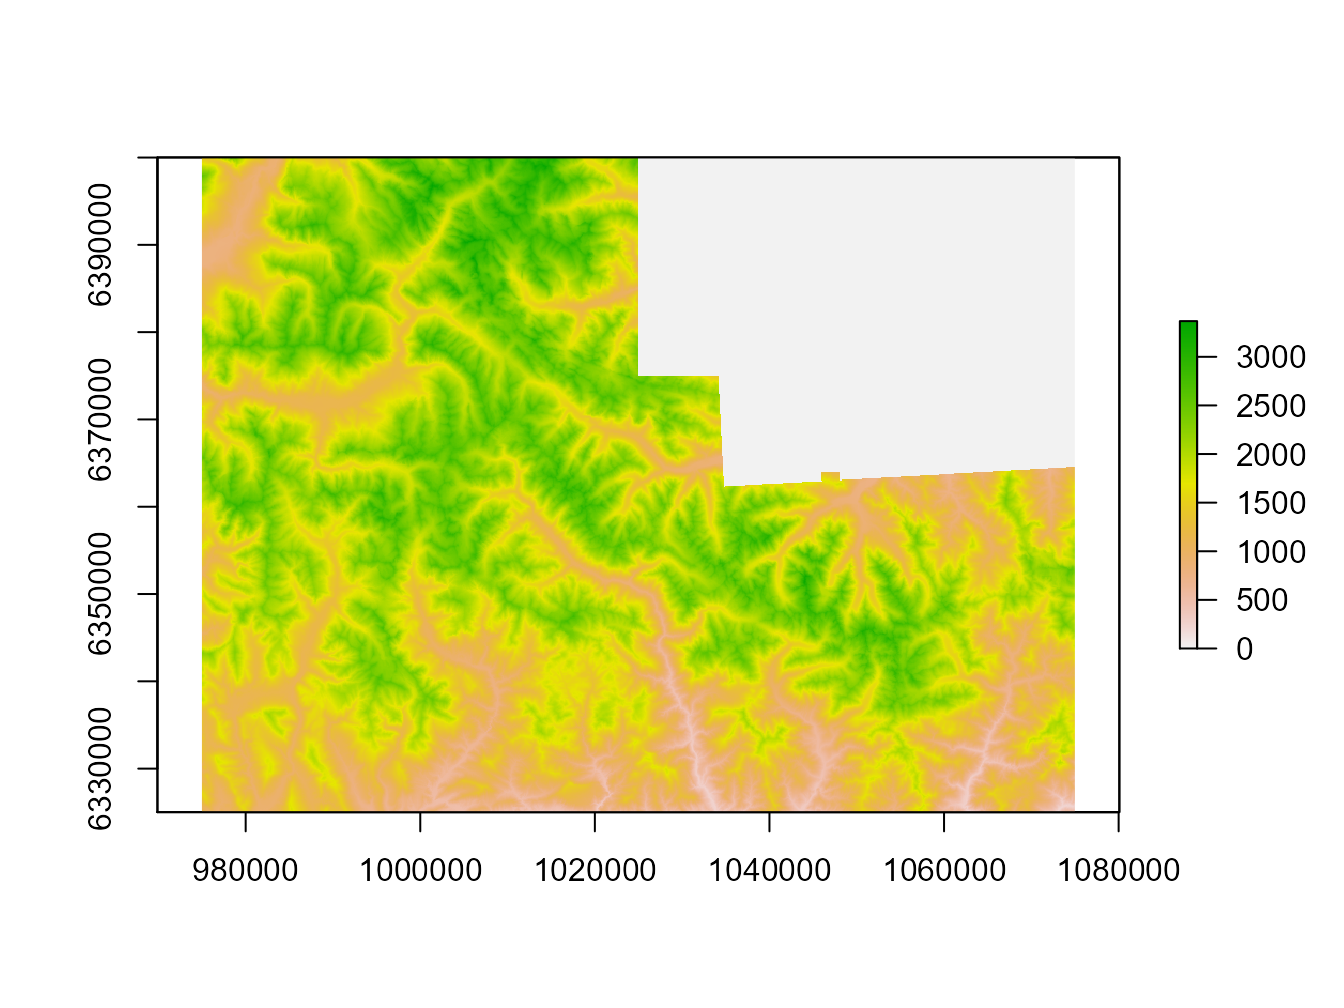
\includegraphics[width=0.8\linewidth]{MyBook_files/figure-latex/MNT-1} \end{center}

\normalsize

\hypertarget{pruxe9sentation-de-la-ptr-tof-ms}{%
\chapter{Présentation de la PTR-ToF-MS}\label{pruxe9sentation-de-la-ptr-tof-ms}}

De très nombreux projets de recherche issus du CeMEB nécessitent l'analyse de \textbf{C}omposés \textbf{O}rganiques \textbf{V}olatils (COV ou VOC en anglais) aussi communément appelés ``odeurs''. Les COVs sont omniprésents dans la nature et permettent, avec les autres sens, une organisation du vivant en agissant comme vecteur d'information de la médiation chimique. Par l'acquisition d'un PTR-ToF-MS, la communauté souhaitait lever trois verrous techniques :

\begin{itemize}
\tightlist
\item
  l'appareil permet un fonctionnement en flux continu avec une résolution temporelle très fine (fréquence d'analyse allant jusqu'à 10 scans par seconde), permettant ainsi le suivi des cinétiques d'émissions de COV. Cet instrument simplifie drastiquement et affine les expériences cinétiques effectuées par des mesures moyennées de GC-MS;\\
\item
  le PTR-ToF-MS possède une excellente résolution en masse qui facilite l'identification des molécules. Un \textbf{spectre} est composé de plus de 140 000 mesures de masses couvrant une large gamme des masses des COV biologiques (de 70 à 500 m/z). L'appareil possède donc une résolution environ mille fois supérieure par rapport à un simple quadripôle (PTR-MS ou GC-MS) qui fournit des m/z à l'unité de masse atomique (uma ou Dalton Da);\\
\item
  le seuil de détection extrêmement bas, de l'ordre du ppt (part per trillion), permet une sensibilité adaptée à la mesure de traces.
\end{itemize}

\hypertarget{une-bruxe8ve-histoire-de-la-ptr-tof-ms}{%
\section{Une brève histoire de la PTR-ToF-MS}\label{une-bruxe8ve-histoire-de-la-ptr-tof-ms}}

Durant la décennie 1990, l'\emph{Institut für Ionenphysik der Leopold-Franzens-Universität} d'Innsbruck en Autriche développe un nouvel instrument pour l'analyse chimique des gaz. En travaillant avec la \emph{Universitiitsklinik fiir Innere Medizin}, l'équipe menée par Lindinger développe un spectromètre en phase gazeuse qui ionise les molécules grâce à un gaz neutre (\autocite{lindinger_1991} et \autocite{lindinger_1993}). Ils comprennent rapidement l'avantage d'utiliser un proton (apporté à la réaction sous la forme H\textsubscript{3}O\textsuperscript{+}) par rapport aux ions Kr\textsuperscript{+} et Xe\textsuperscript{+}. Ils publient une sorte de preuve de concept en 1994 \autocite{lagg_1994} et détaillent plus finement l'instrumentation et les réactions chimiques \autocite{hansel_1995}\footnote{avec des remerciements incroyables}. En 1998 sort l'article qui fait désormais référence, \autocite{lindinger_1998a}, signé par le trio Lindinger, Hansel et Jordan (et sa version courte \textcite{lindinger_1998}).

Ionicon commercialise la même année le premier PTR-MS. Cette technique se déploie rapidement dans les sciences de l'atmosphère, médicales et biotech (\autocite{babcock_2001}) permettant la détection de traces de COV. Rapide et sensible, la PTR-MS élimine certains désavantages de la GC-MS. Cependant, la PTR-MS détecte de la masse nominale des ions. Un échantillon complexe peut contenir plusieurs ions isobares\footnote{molécules possédant un nombre de nucléons identique.}. Il convient alors de gagner en résolution de masse et séparer ces isobares. \autocite{jordan_2009} revient sur les tentatives les plus concluantes (\autocite{blake_2004}, \autocite{ennis_2005}, \autocite{inomata_2006} et \autocite{tanimoto_2007} ) avant de proposer son approche : la PTR-ToF-MS. Développé en collaboration avec la précédente équipe, le minutieux article de \autocite{graus_2010} conclu superbement la vingtaine d'années de développement nécessaire à cette technique. Les années suivantes permettront simplement une amélioration des différentes parties de l'instrument.

Par ailleurs, c'est au tour des mathématiciens d'apporter leur contribution et en particulier à l'équipe de Cappellin avec deux articles. Le premier, \autocite{cappellin_2010}, permet de mieux estimer la masse exacte de chaque ion détecté. Le seconde, \autocite{cappellin_2011}, offre une méthodologie détaillée de l'utilisation du PTR-ToF-MS de l'acquisition à la fin de l'analyse. Puis en 2015, \autocite{holzinger_2015} propose un logiciel pour l'analyse des data mais cette tentative n'a pas été suivie par la communauté d'utilisateurs. Il existe désormais un nombre important d'articles utilisant la PTR-ToF-MS. Bien entendu, des outils communs de chimiométrie ont été utilisés pour renforcer les résultats, \autocite{deuscher_2019}. Mais cela sera abordé dans le chapitre suivant.

Je suppose que la prochaine avancée majeure viendra d'une technologie permettant de discriminer les isomères\footnote{molécules partageant la même formule brute mais avec un agencement tridimensionnel différent.} \autocite{amt-14-133-2021} \footnote{si un mémoire de master permettait la science fiction, j'aurais évidemment développé quelques idées à propos de capteurs de champs électromagnétiques ou de spectromètres optiques à la place des capteurs MS actuels.}. Par exemple, cela permettrait de séparer les différents monoterpènes omniprésents dans les émissions végétales et qui nous concernent particulièrement en écologie chimique. Actuellement, ce désavantage est comblé par le couplage de la PTR-ToF-MS avec une seconde technique d'analyse chimique. Ce court historique montre toutefois que la collaboration entre physiciens, chimistes, biologistes et mathématiciens est fructueuse et promise à un bel avenir.

\hypertarget{instrumentation-guxe9nuxe9rale}{%
\section{Instrumentation générale}\label{instrumentation-guxe9nuxe9rale}}

\begin{figure}
\hypertarget{fig:schemavocus}{%
\centering
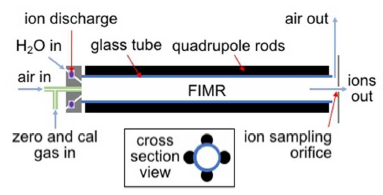
\includegraphics{images/schema_vocus.PNG}
\caption{Schéma de la chambre d'ionisation (Reprinted with permission from \textcite{krechmer_2018}. Copyright 2021 American Chemical Society.)}\label{fig:schemavocus}
}
\end{figure}

Comme nous l'avons vu précédemment, le PTR-ToF-MS est conçu pour analyser finement la masse moléculaire des échantillons. Pour cela l'instrument aspire un débit d'air constant de 100 ml/min\footnote{ou sccm, pour \emph{standard cubic centimeters per minute}}. Cet \emph{air in} sur la figure \ref{fig:schemavocus} peut être connecté à un gaz zéro pour diluer un échantillon trop concentré (pour éviter la saturation) ou à un gaz étalon pour l'étalonnage de l'instrument. Le flux d'air est ensuite injecté dans le réacteur (\emph{FIMR} pour \emph{focusing ion-molecule reactor}). Dans cette chambre, des ions H\textsuperscript{+} issus d'eau ultra pure sont également injectés à débit constant afin d'ioniser les molécules de l'échantillon (\emph{Proton-Transfer-Reaction}).

Il est important de comprendre que, contrairement à une ionisation par électron\footnote{comme c'est le cas en ionisation électronique fréquemment utilisée en GC-MS.}, il n'y a quasiment pas de fragmentation moléculaire. C'est une ionisation douce, comme en ESI (ElectroSpray Ionization) fréquemment utilisée en LC-MS. Les ions ont ``une unité de masse molaire de plus''(un proton) que les ions moléculaires. Par exemple, le linalol, un COV fortement produit par la lavande, a une masse molaire de 154,249 g/mol mais sera detecté à 155,256 g/mol. Par ailleurs, le nombre d'ions MH\textsuperscript{+} détectés dépend du taux de protonation de la molécule M. Sous forme d'ions, l'échantillon peut être focalisé par un champ électromagnétique généré par un quadripôle et envoyé dans la partie ToF.

Une fois dans la colonne, l'énergie potentielle d'un pulse électromagnétique à 25kHz est convertie en énergie cinétique par les ions propulsés. À énergie constante, la masse fait la différence lors de la mesure du temps de vol (ToF, figure \ref{fig:schemaToF}). Ainsi les ions les moins lourds arrivent en premiers sur le détecteur. Le comptage du nombre de coups sur le détecteur donne l'intensité par unité de temps. Un étalonnage, avec des ions moléculaires étalons, permet de convertir le \emph{temps de vol} en \emph{masse}, ce qui permet par la suite d'analyser les masses des échantillons inconnus.

\begin{figure}
\hypertarget{fig:schemaToF}{%
\centering
\includegraphics{images/schema_TOF.jpg}
\caption{Schéma de la colonne ToF et du détecteur MS (Reproduit de l'article \textcite{graus_2010})}\label{fig:schemaToF}
}
\end{figure}

Pour une compréhension plus exhaustive, je recommande la lecture des articles de \textcite{hansel_1995} pour la partie PTR-MS, de \textcite{graus_2010} pour la partie ToF et de \textcite{krechmer_2018} spécifique à l'instrument utilisé au CEFE.

\hypertarget{analyse-et-conclusion}{%
\section{Analyse et conclusion}\label{analyse-et-conclusion}}

\hypertarget{le-plan-dexpuxe9rience}{%
\subsection{Le plan d'expérience}\label{le-plan-dexpuxe9rience}}

Pour illustrer cela, je présenterais une expérience sur les lavandes. Cette expérience s'inscrit dans un cadre d'un projet MUSE (Montpellier Université d'Excellence) porté par Magali Proffit et s'intéressant aux phénomènes de pollution à l'Ozone O\_3 liés au changement climatique global. Nous nous sommes intéressés aux variations journalières des émissions de COV de lavandes isolés dans des chambres de prélèvements. Les acquisitions se déroulaient durant 48h à cheval sur trois jours et deux nuits afin de décrire le rythme circadien des plantes.

Nous avons mis en place quatre chambres de mesure permettant chacune soit d'isoler un plant de lavande soit d'être un blanc. Ces chambres de mesure sont des cylindres en plastique, ventilés, de volumes équivalents et reliés à un flux d'air zéro d'un débit de 5 litres/min. La longueur et le volume des lignes reliant les chambres à l'instrument de mesure n'étaient pas identiques. Nous avons lancé des acquisitions sur les quatre chambres séquentiellement durant 48h. Nous avons répété ce processus deux fois, pour obtenir neuf plants au total dans notre plan d'expérience (cf.~\ref{tab:PlanXP}).

\scriptsize

\normalsize

\hypertarget{ruxe9sultats-de-la-mcr}{%
\section{Résultats de la MCR}\label{ruxe9sultats-de-la-mcr}}

\scriptsize

\begin{figure}

{\centering 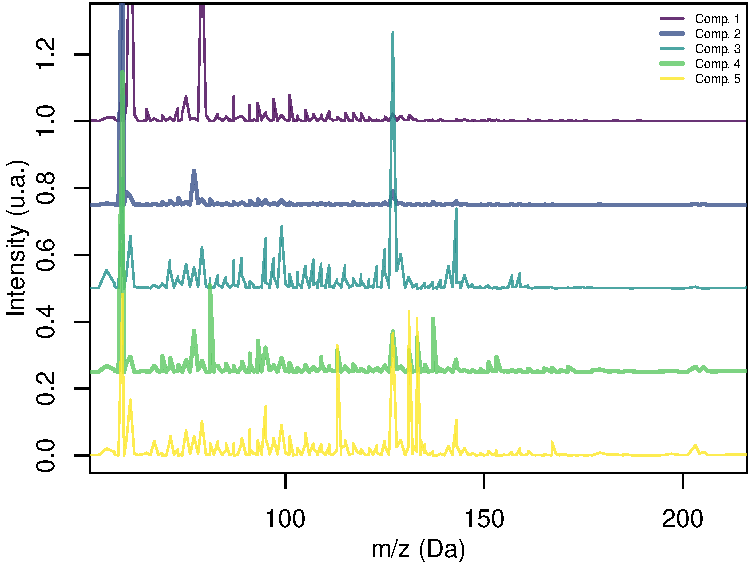
\includegraphics[width=0.8\linewidth]{MyBook_files/figure-latex/MCRloadings-1} 

}

\caption{Spectres purs, loadings MCR}\label{fig:MCRloadings}
\end{figure}

\normalsize

\scriptsize

\begin{figure}

{\centering 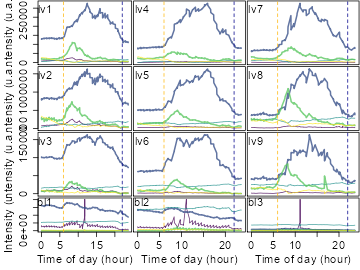
\includegraphics[width=0.8\linewidth]{MyBook_files/figure-latex/MCRscores-1} 

}

\caption{Evolution cinetique des spectres purs}\label{fig:MCRscores}
\end{figure}

\normalsize

Les spectres issus de ces expériences sont ensuite analysés avec des outils de chimiométrie pour explorer au maximum toute la complexité des données à traiter. Certains algorithmes, comme la MCR-ALS, permettent le développement de modèles multivoies pour prendre en compte l'aspect cinétique de la PTR-ToF-MS.

J'ai utilisé l'algorithme de la MCR-ALS pour décomposer le spectre total en spectres purs( \ref{fig:MCRscores} ). Ces spectres purs sont des ensembles de COV représentatifs d'un phénomène propre. En optimisant la MCR-ALS, j'ai fait ressortir, entre autres, l'évolution de deux spectres purs montrant un double cycle d'émission journalier ( \ref{fig:MCRscores} ). La première activité intervient peu après l'aube, atteint un pic d'émission autour de 8h et diminue rapidement pour retrouver un niveau comparable au niveau initial vers midi. La seconde activité plus tardive augmente jusqu'à un plateau atteint vers midi et se prolonge jusqu'à 16h pour décroître par la suite.

\newpage

\hypertarget{bibliographie}{%
\section{Bibliographie}\label{bibliographie}}

This template is based on \emph{Bookdown} and the \emph{Memoir} LaTeX class to allow writing a book, a report, a PhD thesis, etc. in \emph{R Markdown}.

The main file is \emph{index.Rmd} which contains the description of the book in its header. All other \emph{.Rmd} files in the folder contain a chapter.
The \emph{references.bib} file contains the bibliography.

This file will have to be deleted, as well as \emph{81-getting\_started.Rmd} and \emph{82-syntax.Rmd}: they have to be replaced by the content of the book.

To get started, create a new R project from this folder.
Then open \emph{index.Rmd} and click on the \emph{Build Book} button in the \emph{Build} window of Rstudio.


% Bibliography
%%%%%%%%%%%%%%%%%%%%%%%%%%%%%%%%%%%%%%%%%%%%%%%%%%%%%%%%%%

\backmatter
\SmallMargins

\printbibliography
\onecolumn


% Tables (of tables, of figures)
%%%%%%%%%%%%%%%%%%%%%%%%%%%%%%%%%%%%%%%%%%%%%%%%%%%%%%%%%%


\cleardoublepage
\LargeMargins
\listoffigures


% After-body (LaTeX code inclusion)
%%%%%%%%%%%%%%%%%%%%%%%%%%%%%%%%%%%%%%%%%%%%%%%%%%%%%%%%%%




% Back cover
%%%%%%%%%%%%%%%%%%%%%%%%%%%%%%%%%%%%%%%%%%%%%%%%%%%%%%%%%%%

% Even page, small margins, no running head, no page number.
\evenpage
\SmallMargins
\thispagestyle{empty}

\begin{normalsize}

\begin{description}

\selectlanguage{english}
\item[Abstract]
English abstract, on the last page.

This is a bookdown template based on LaTeX memoir class.
\item[Keywords]
Keyword in English, As a list.
~\\

\end{description}

\end{normalsize}

\vspace*{\fill}
\centering
\includegraphics[width=.3\textwidth]{images/logo}
\end{document}
